\documentclass[10pt]{article}

\title{ITF31519 - Assignment 3}
\author{Tobias Hallingstad and Mathias Mellemstuen}

\usepackage[utf8]{inputenc}
\usepackage[english]{babel}
\usepackage{minted}
\usepackage[T1]{fontenc}

\usepackage{graphicx}

\usepackage{graphicx}
\graphicspath{ {./images/} }

\begin{document}
    \begin{titlepage}
        \maketitle
    \end{titlepage}

    \newminted{python}{
        gobble=2,
        linenos
    }

    \section{Load and prepeareing the data}
    To load the data we use \texttt{pandas}. We read all the data from the training and test data set. Afther looking at the data we also see that coloum 1 is a ID feald, so we remove that coloum.

    \begin{pythoncode}
    trainingData = pd.read_csv("ALS_TrainingData_2223.csv").drop('ID', axis=1)
    testingData = pd.read_csv("ALS_TestingData_78.csv").drop('ID', axis=1)
    \end{pythoncode}

    \section{Preforming summary and preliminary visulization}
    Using \texttt{pandas dataframe.info()} we see that the data contiauns 100 diffrent classes. The data is only a combination of ints and floats. There are 2223 diffrent elements in the training data, while the test data contains 78 elements. This is wiht the \texttt{ID} feald removed. 

    \section{Normalize the data, and analyzation of the data}
    To normalize the data we use a function we created. To make is simpler to normalize the data for training and test data. The function is called \texttt{normalizePCAData()}. This function takes \texttt{data} and \texttt{components} as parameters. \texttt{data} is the dataframe with the data. \texttt{components} is the dimention the data is going to be reduced to.

    The normalization function is pretty simple. First we initilize a \texttt{StandardScaler()} object. This is used in the \texttt{scalar.fit\_transform(data)} method. Then the data is normalized using the \texttt{normalize()} functuion. Bouth of these functions are from \texttt{sklearn.preprocessing}.

    Afther all of this we can see that the data looks like this:

    \begin{center}
        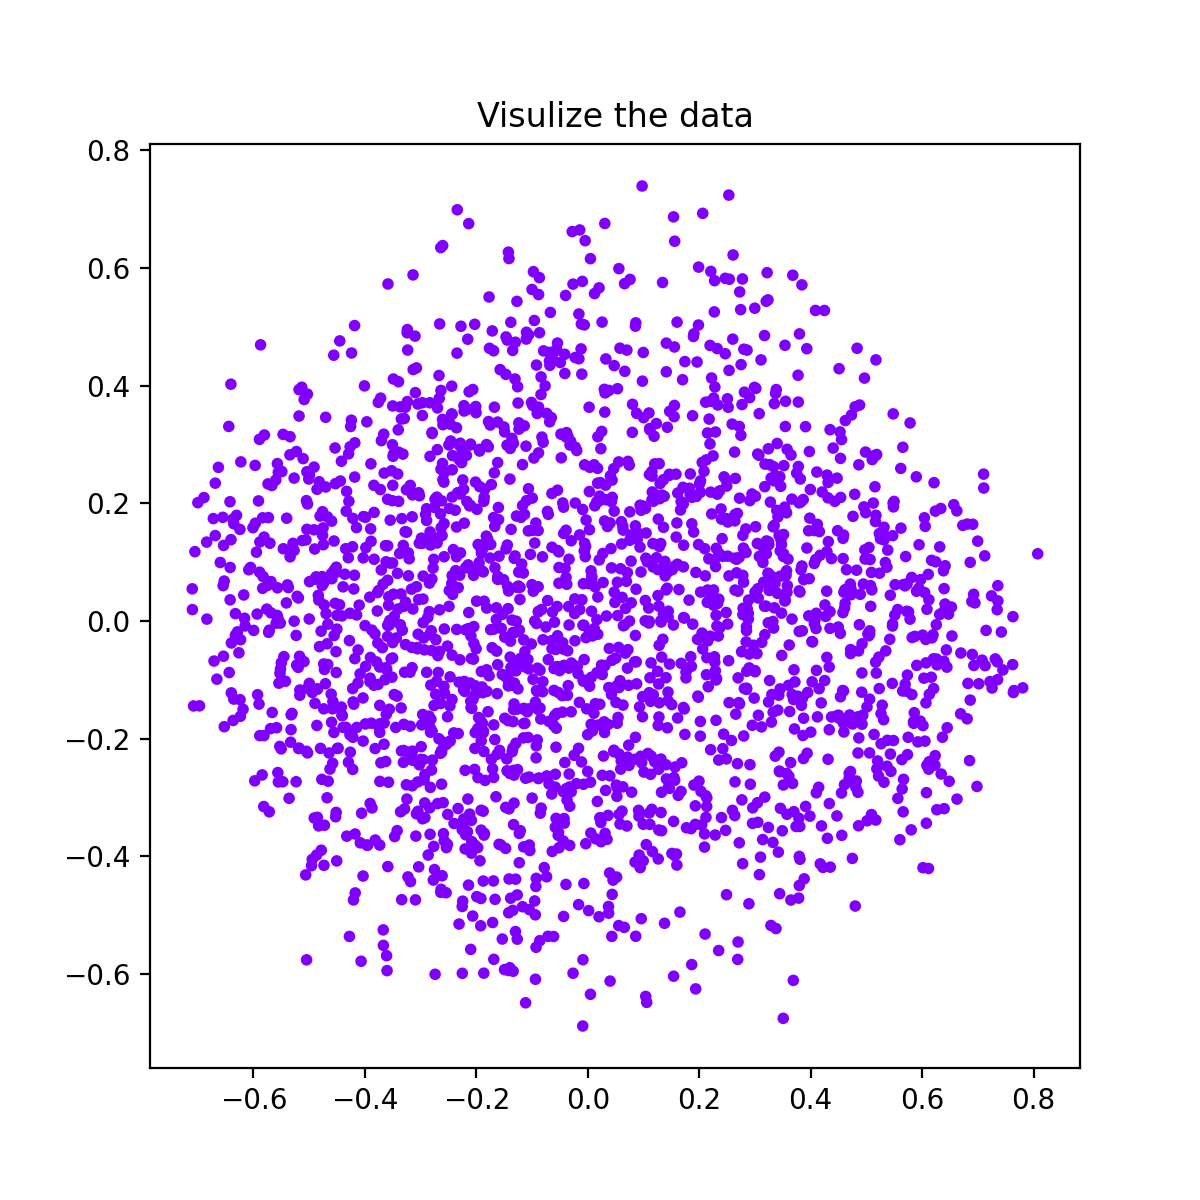
\includegraphics[scale=0.5]{Figure_1.png}
    \end{center}

    \section{K-means clustering}
    One way to find the value of \texttt{K} could be to look at the data. But when looking at this data we do not see a clear way to categorize the data. So we can do multiple things.

    To run the code with K number of klusters use this code: 

    \begin{pythoncode}
        $ python task.py <plot_type> <K>
    \end{pythoncode}

    \paragraph{Square root}
    One way to find how many classes there should be is to take the square root of the amount datapoints in the datasett. Even though this is ment for K-NN we can stil try it for K-means. We do have 2223 points of data. That makes:
    
    \[K = \sqrt{2223} = 47\]

    We then try to run a scatter plot of this to see what we get. To see if this is a "good" sulution we will find out by looking at the other methods.

    \begin{center}
        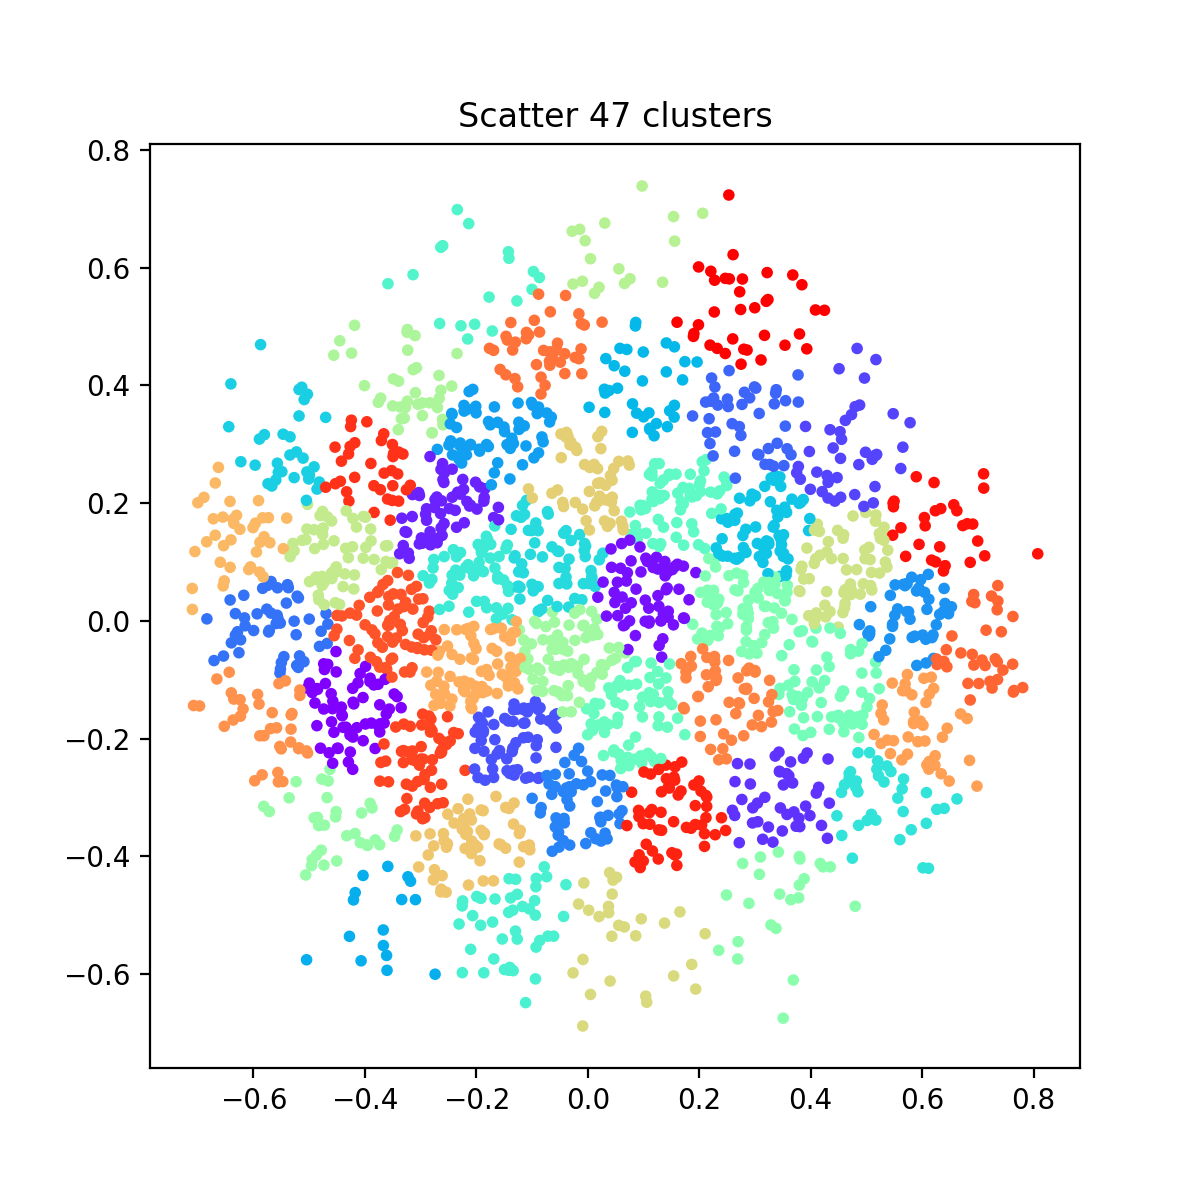
\includegraphics[scale=0.5]{scatter_47.png}
    \end{center}

    Afther printing the number of items in each cluster. We see that the spread is very large. Indicationg that the clustering might not be the best. When thingink about how the data looks. 

    \paragraph{Dendogram}
    We can try to draw a dendogram of the clustering and se if we find som good cutoff point.

    \begin{center}
        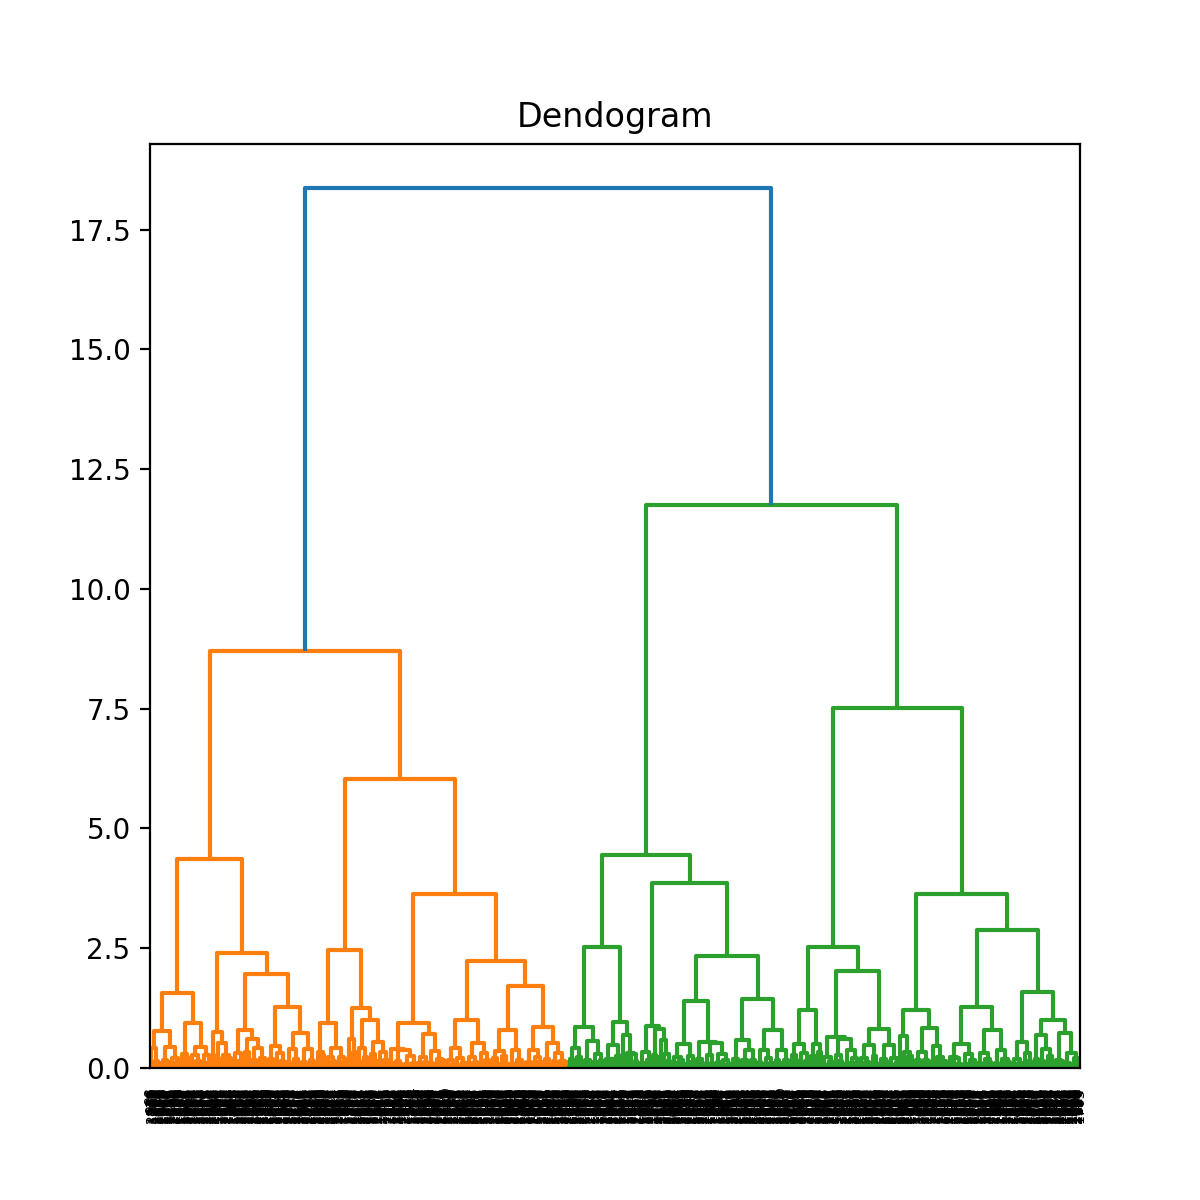
\includegraphics[scale=0.5]{dend.png}
    \end{center}

    Looking at this we see that a K of 2-3 migth be a good value. 

    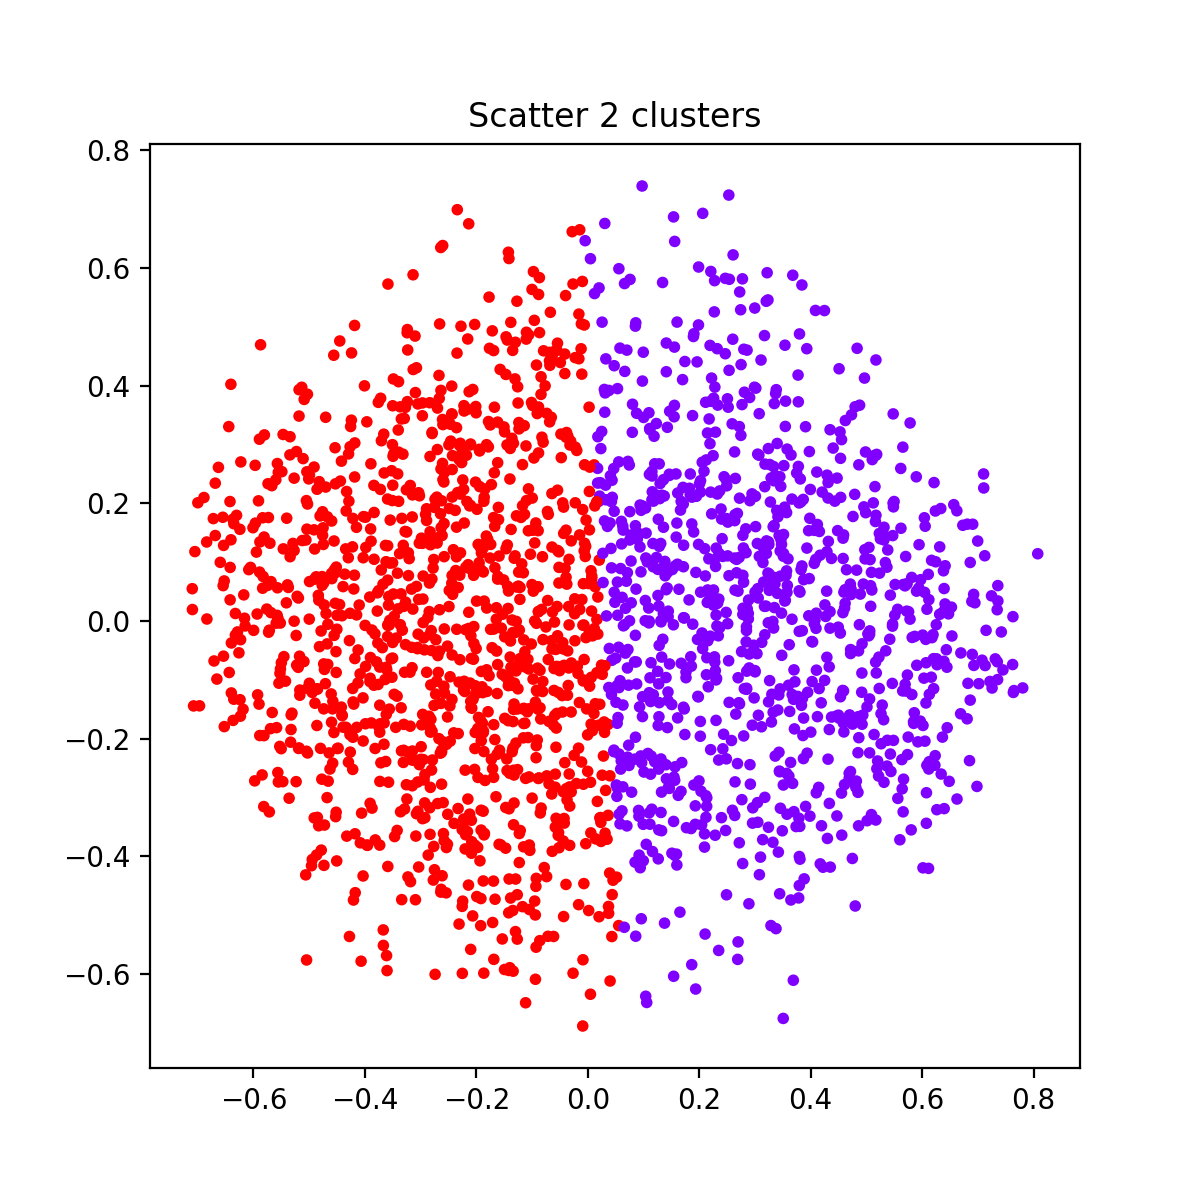
\includegraphics[scale=0.35]{scatter_2.png}
    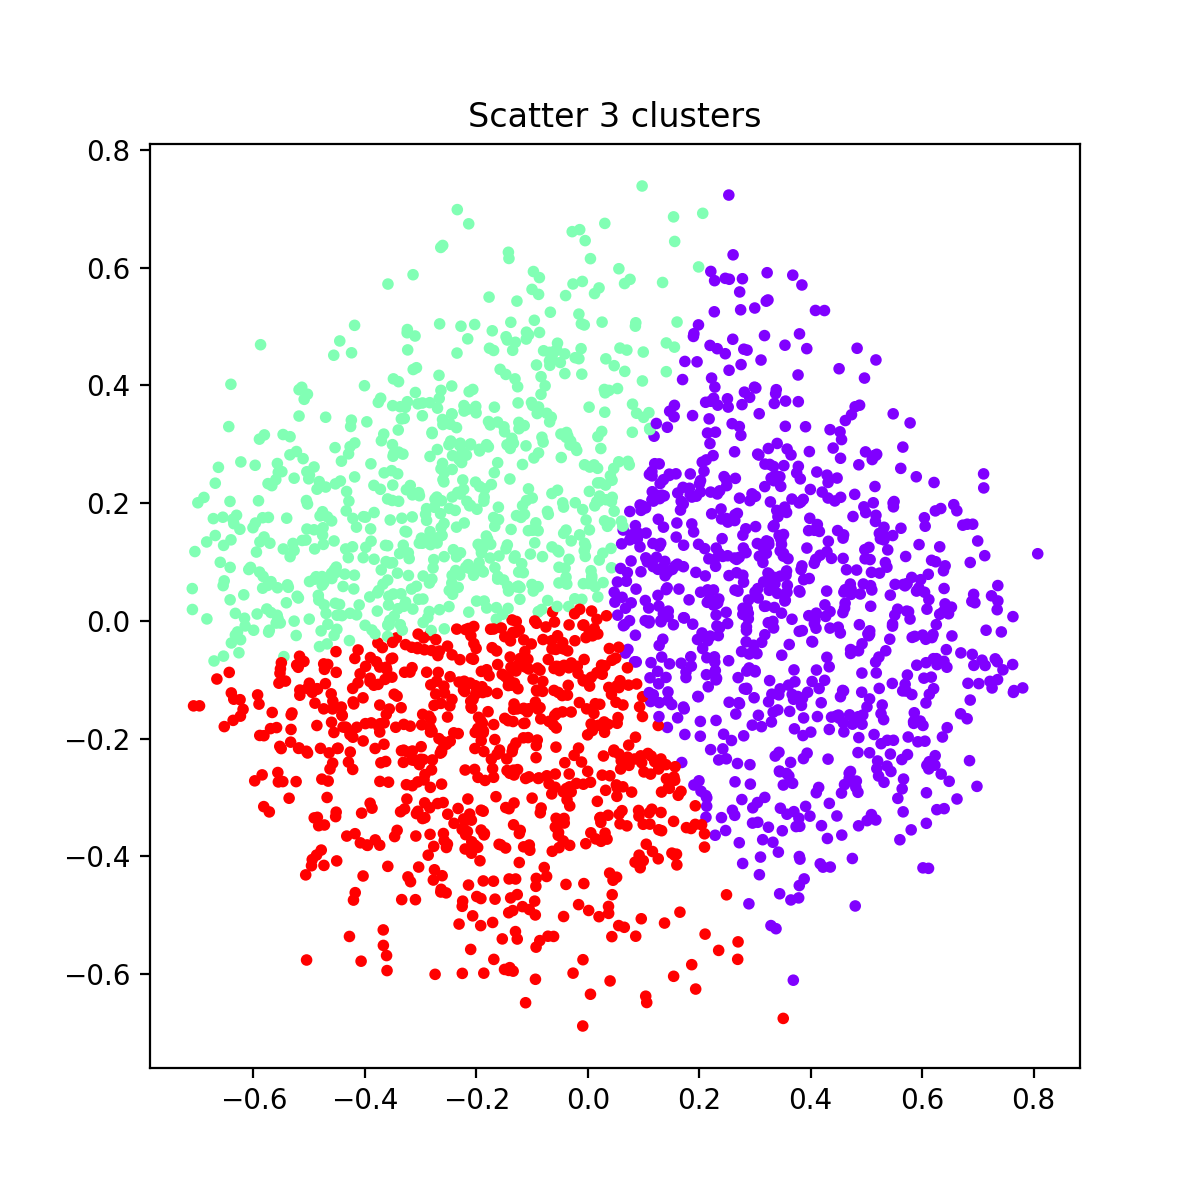
\includegraphics[scale=0.35]{scatter_3.png}

    For a 2 clusters we see that we get around 200 items more in one cluster then the other. While for 3 clusters we see that the total is also around 200, but each step is around 100. This can probaly indicate that this is to few clusters.
    
    \paragraph{Elbow}
    Here we calculate the WSS (Within-Cluser-Sum of Squared errors). We calculate this for diffrent K untill we see that WSS starts become the same value. To do this we just calculate the WSS from K = 1 to 100 and plot the resoult in a line diagram.

    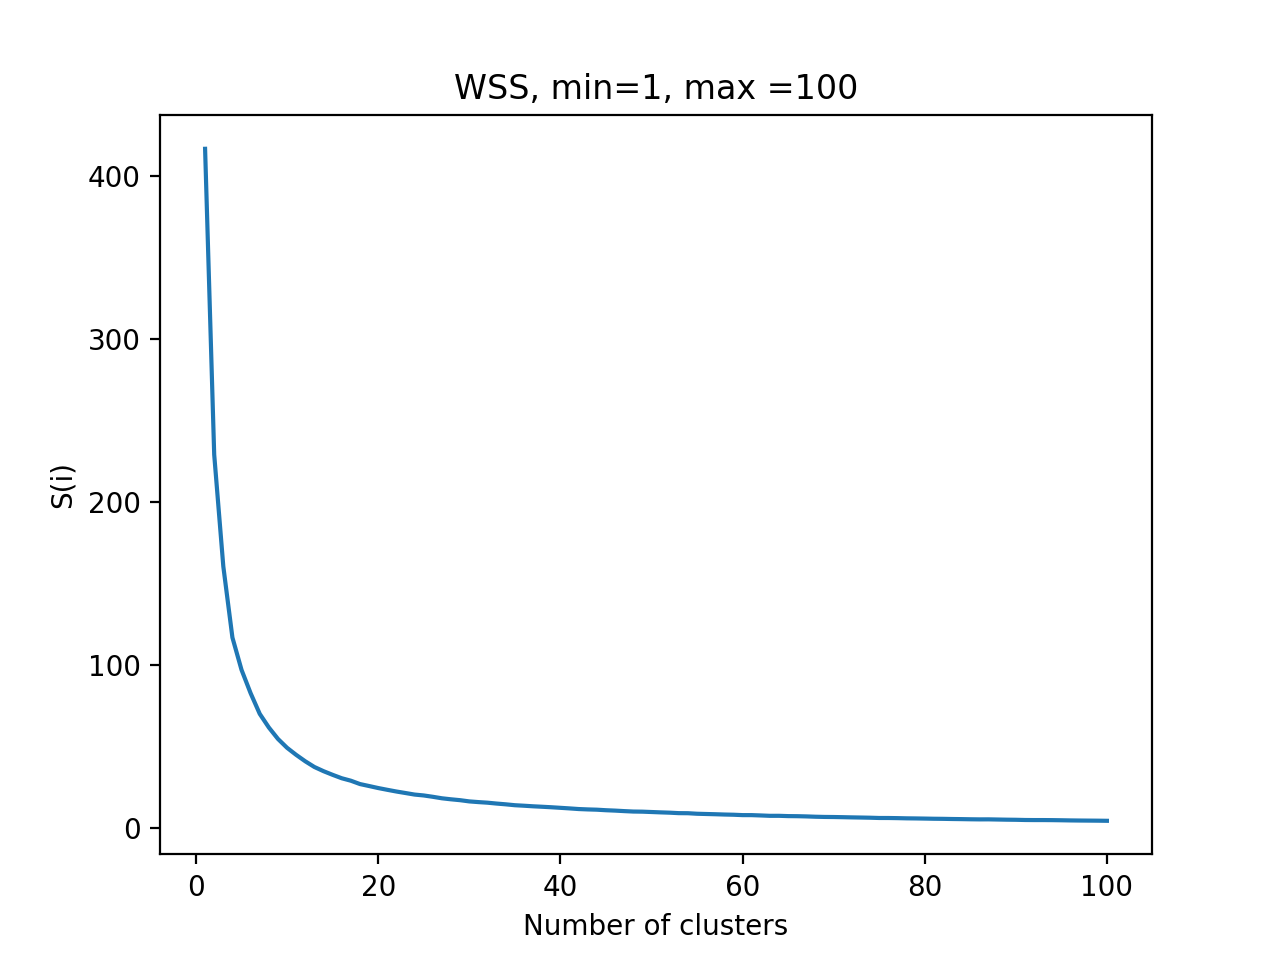
\includegraphics[scale=0.35]{wss_line_100.png}
    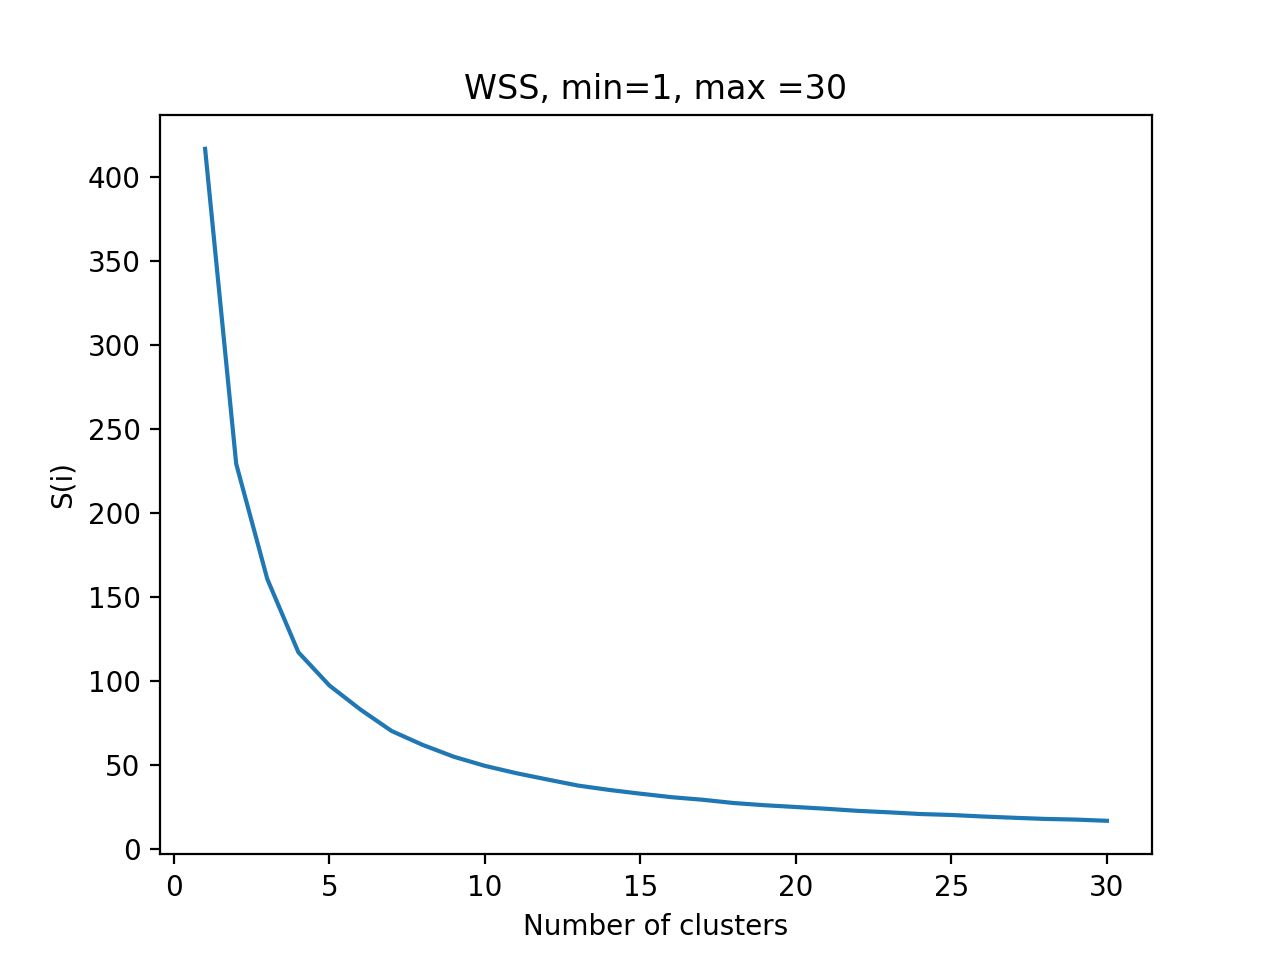
\includegraphics[scale=0.35]{wss_line_30.png}

    From what we can see here something around 5-10 seems like a good K. Doing a quick look at the number of items in the diffrent models, from 5 to 10 clusters. We can see that clusters in the lower range can give a smaller variance then the upper cluster might. This can indicate that something closer to 5 might be optimal.

    \paragraph{Slihouette}
    We can also use the Slihouette method. This method messures how simular a value is to another its cluster, compeard to other clusters. We try with the same values as with elbow to see if we get the same number for K or somethig diffrent.

    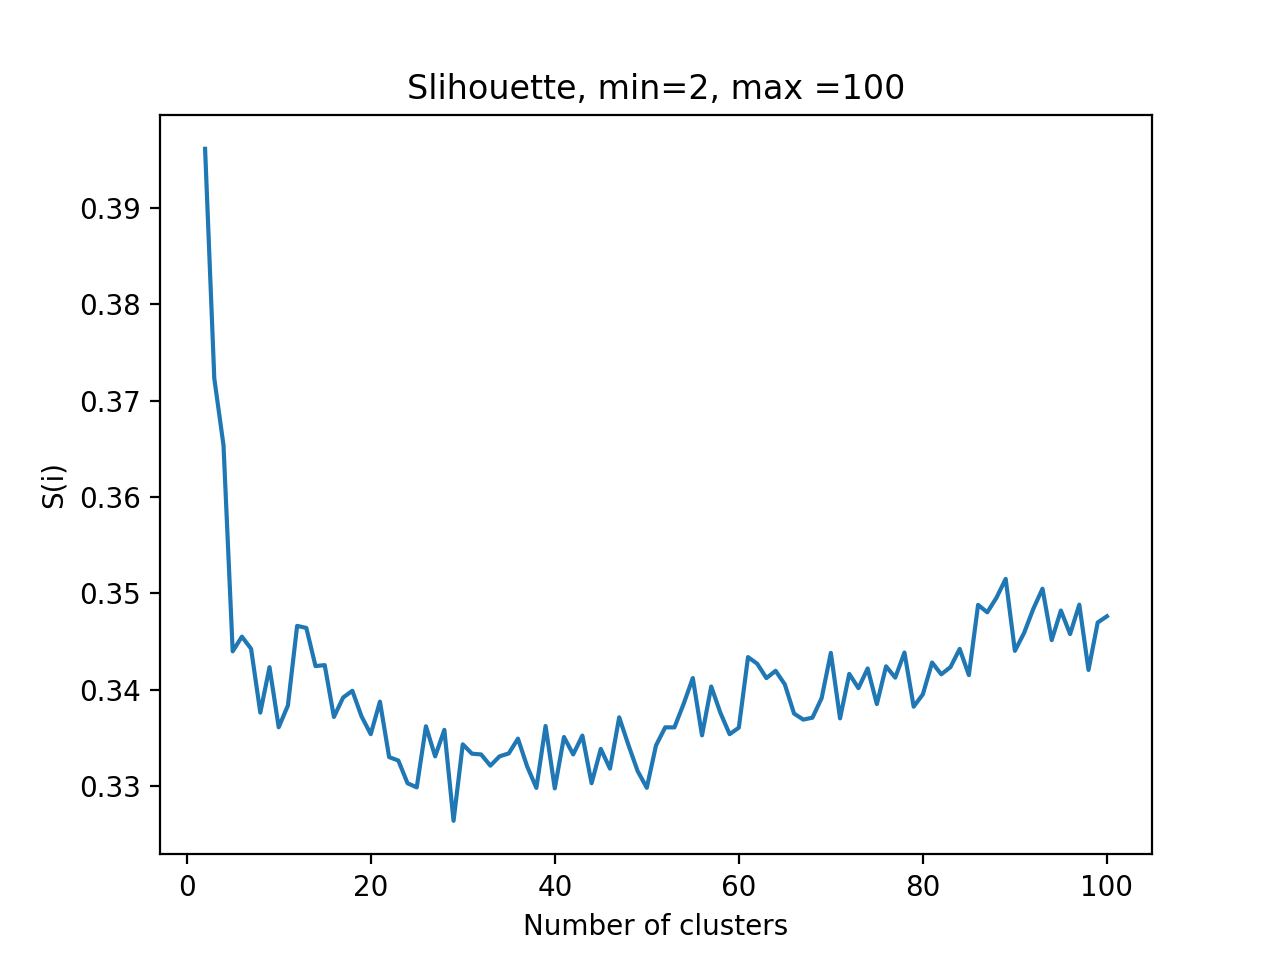
\includegraphics[scale=0.35]{slih_line_100.png}
    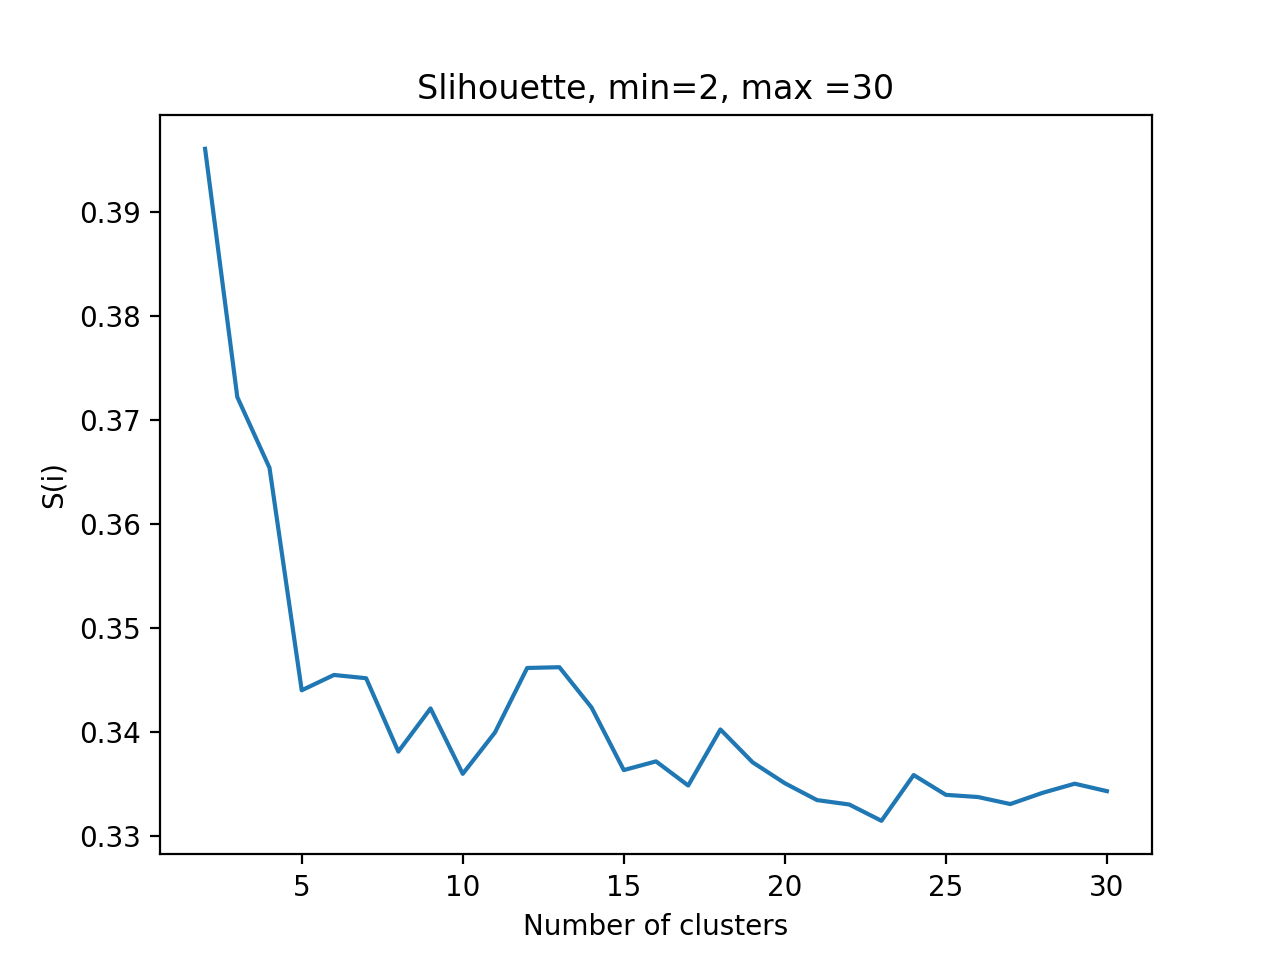
\includegraphics[scale=0.35]{slih_line_30.png}

    From what we see K = 6 seems like a good K too use in for this model. If we plot this in a scatter diagram we get this:

    \begin{center}
        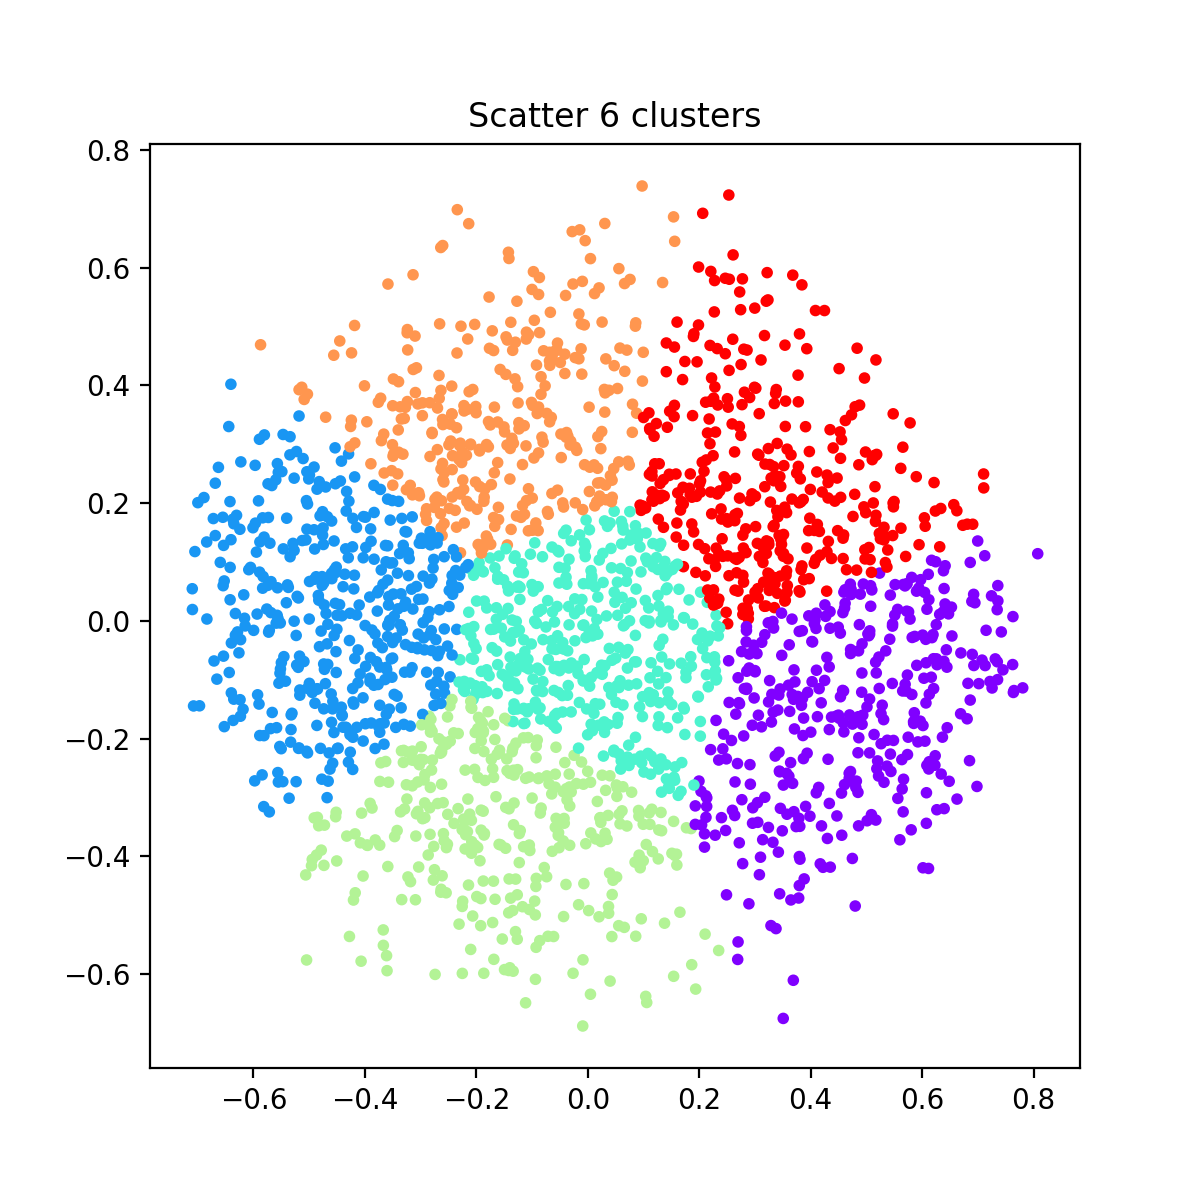
\includegraphics[scale=0.5]{scatter_6.png}
    \end{center}

    For K = 6 we can see that we have a diffrence of about 95 items. The cluster with the items seems the mostly the same also. This can indicate that this is a good K for this dataset. From the scatter plot we can also see that we get a nice lable area.

    \section{Conclution}
    We can see that for trying to label large data sets there are many diffrent ways of findng out how many clusters there needs to be. Some methods are easy to calculate, but end up over or under doing how many clustesr are needed. The more advanced the way of finding K is, the better the estimation will be. 

    Using the slihouette methode worked realy well on this data set. By using some manual work at the end to find the "perfect" number for K, we can se that 6 is a good option. Going up or down from there gives some valuse higher that what K=6 gives.

    As always there is no perfect rule to fitt all models. But for this data set it seems like slihouette is a good method.


    \section{Running the code}
    To run the code and get something to print the following commands can be used

    \paragraph{Just run the code}
    \begin{pythoncode}
        $ python task.py
    \end{pythoncode}

    \paragraph{Get a scatter plot of K clusters}
    \begin{pythoncode}
        $ python task.py scatter <K>
    \end{pythoncode}

    \paragraph{Get a dendogram}
    \begin{pythoncode}
        $ python task.py dend
    \end{pythoncode}

    \paragraph{Get scores inside a range of clustes, bar diagram}
    \begin{pythoncode}
        $ python task.py bar <min_cluster> <max_cluster> <Slihouette | wss>
    \end{pythoncode}

    \paragraph{Get scores inside a range of clustes, line diagram}
    \begin{pythoncode}
        $ python task.py line <min_cluster> <max_cluster> <Slihouette | wss>
    \end{pythoncode}

\end{document}